\documentclass[12pt]{article}
\usepackage[margin=2.5cm]{geometry}
\usepackage{enumerate}
\usepackage{amsfonts}
\usepackage{amsmath}
\usepackage{fancyhdr}
\usepackage{amsmath}
\usepackage{amssymb}
\usepackage{amsthm}
\usepackage{mdframed}
\usepackage{graphicx}
\usepackage{subcaption}
\usepackage{adjustbox}
\usepackage{listings}
\usepackage{xcolor}
\usepackage{booktabs}
\usepackage[utf]{kotex}
\usepackage{hyperref}

\definecolor{codegreen}{rgb}{0,0.6,0}
\definecolor{codegray}{rgb}{0.5,0.5,0.5}
\definecolor{codepurple}{rgb}{0.58,0,0.82}
\definecolor{backcolour}{rgb}{0.95,0.95,0.92}

\lstdefinestyle{mystyle}{
    backgroundcolor=\color{backcolour},
    commentstyle=\color{codegreen},
    keywordstyle=\color{magenta},
    numberstyle=\tiny\color{codegray},
    stringstyle=\color{codepurple},
    basicstyle=\ttfamily\footnotesize,
    breakatwhitespace=false,
    breaklines=true,
    captionpos=b,
    keepspaces=true,
    numbers=left,
    numbersep=5pt,
    showspaces=false,
    showstringspaces=false,
    showtabs=false,
    tabsize=1
}

\lstset{style=mystyle}

\pagestyle{fancy}
\renewcommand{\headrulewidth}{0.4pt}
\lhead{CSC 209}
\rhead{Review 4 Solution}

\begin{document}
\title{CSC 209 Review 4 Solution}
\maketitle

\bigskip

\begin{enumerate}[1.]
    \item

    The answer is \texttt{a) *p} and \texttt{g) *\&i}.

    \bigskip

    \underline{\textbf{Notes}}

    \bigskip

    \begin{itemize}
        \item \textbf{Address and Indirection Pointers}

        \begin{itemize}
            \item If \texttt{x} is a variable, \texttt{\&x} points to its memory address
            \item * in \texttt{*p} is called \textbf{Indirection operator}
            \begin{itemize}
                \item Allows variable to gain access to the object pointed by \texttt{p}
            \end{itemize}
        \end{itemize}
        \item \textbf{Aliases}

        \begin{itemize}
            \item Is the situation where the value in same memory location can be accessed using different variable names.

            \bigskip

            \underline{\textbf{Example 1:}}

            \bigskip

            \texttt{int i, p*;\\
            p = \& i;\\
            printf("\%d$\backslash$n", *p); /* *p is an alias of i */}

            \bigskip

            \underline{\textbf{Example 2:}}

            \bigskip

            \texttt{int i, p*;\\
            p = *\&i /* *p is an alias of i */}
        \end{itemize}
    \end{itemize}

    \item

    \bigskip

    The answers are \texttt{b) *p = \&i;}, \texttt{f) p = q;}, and \texttt{i) *p = *q;}

    \bigskip

    \begin{mdframed}
    \underline{\textbf{Correct Solution}}

    \bigskip

    The answers are \color{red}\texttt{e) p = *\&q;}\color{black}, \texttt{f) p = q;}, and \texttt{i) *p = *q;}

    \bigskip

    \color{red}\texttt{p = *\&q;} is the same as \texttt{p = q}\color{black}

    \end{mdframed}

    \underline{\textbf{Notes}}

    \begin{itemize}
        \item The \texttt{*} operator turns a \textit{value} of type \texttt{pointer to T} into a \textit{variable} of type \texttt{T}.
        \item The \texttt{\&} operator turns a \textit{variable} of type \texttt{T} into a \textit{value} of type pointer to \texttt{T}.
        \item \textbf{Pointer Assignment}

        \begin{itemize}
            \item The following is an example of correct pointer assignment

            \bigskip

            \texttt{int i, j, *p. *q;\\
            p = \&i;
            }

            \bigskip

            \begin{itemize}
                \item Means the memory address of \texttt{p} is pointing to memory address of \texttt{i}
            \end{itemize}

            \bigskip

            \item The following is another valid example of pointer assignment

            \bigskip

            \texttt{int i, j, *p. *q;\\
            p = \&i;\\
            q = p;
            }

            \bigskip

            \begin{itemize}
                \item Means memory address of \texttt{q} is the memory address of \texttt{p} (which is the memory address of \texttt{i})
            \end{itemize}

            \begin{center}
            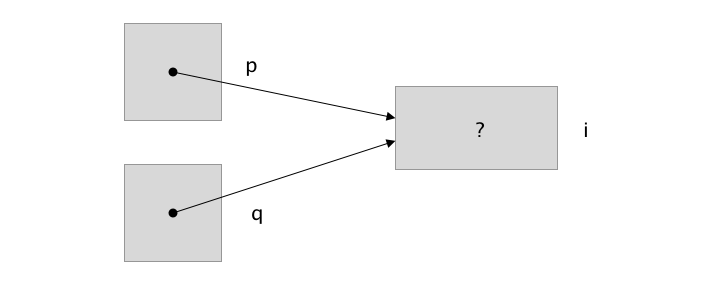
\includegraphics[width=0.6\linewidth]{images/review_4_solution_1.png}
            \end{center}

            \bigskip

            \texttt{*p = 1;}

            \begin{center}
            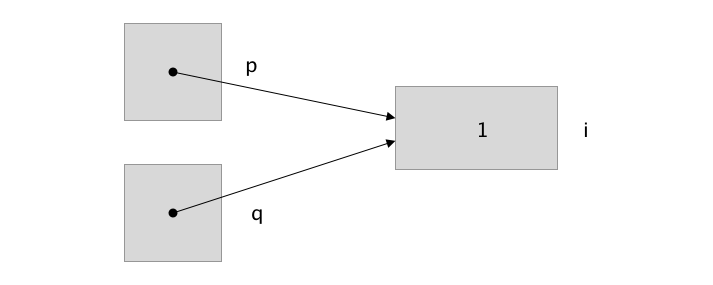
\includegraphics[width=0.6\linewidth]{images/review_4_solution_2.png}
            \end{center}

            \bigskip

            \texttt{*p = 2;}

            \begin{center}
            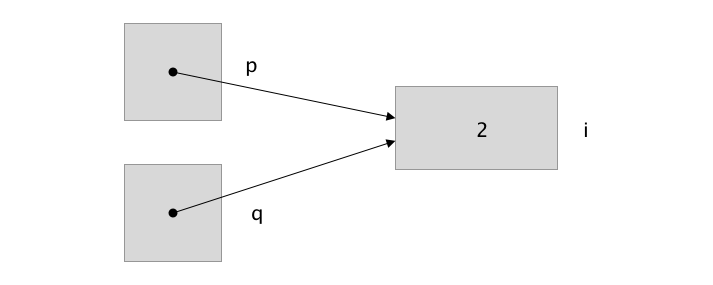
\includegraphics[width=0.6\linewidth]{images/review_4_solution_3.png}
            \end{center}

            \item The following is not a pointer assignment

            \bigskip

            \texttt{*q = *p}

            \begin{itemize}
                \item It \underline{copies the value that} \texttt{p} points to
            \end{itemize}

            \begin{center}
            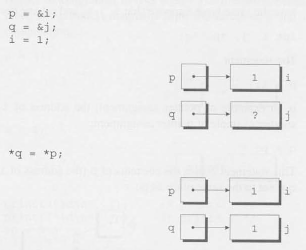
\includegraphics[width=0.6\linewidth]{images/review_4_solution_4.png}
            \end{center}

        \end{itemize}
    \end{itemize}

    \item

    \bigskip

\begin{lstlisting}[language=c]
    void avg_sum(double a[], int n, double *avg, double *sum)
    {
        int i;

        *sum = 0.0;
        for (i = 0; i < n; i++)
            *sum += a[i];
        *avg = *sum / n;
    }
\end{lstlisting}

    \bigskip

    \underline{\textbf{Notes:}}

    \begin{itemize}
        \item \textbf{Pointer as Arguements:}

        \begin{itemize}
            \item Construct protype using pointer variable as parameter
            so it can be passed by refernce

            \bigskip

            \underline{\textbf{Example}}

            \bigskip

            \begin{center}
            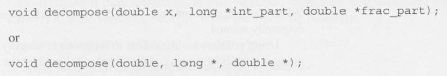
\includegraphics[width=\linewidth]{images/review_4_solution_5.png}
            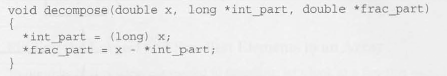
\includegraphics[width=\linewidth]{images/review_4_solution_7.png}
            \end{center}

            \bigskip

            \item When using the prototype, pass variable to prototype by reference
            using \& operator (points to variable's memory location)

            \begin{center}
            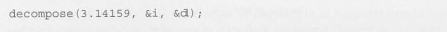
\includegraphics[width=\linewidth]{images/review_4_solution_6.png}
            \end{center}

            \bigskip
        \end{itemize}
    \end{itemize}

    \item

\begin{lstlisting}[language=c]
    void swap(int *p, int *q) {
        int temp;

        temp = *p;
        *p = *q;
        *q = temp;
    }
\end{lstlisting}

    \item

\begin{lstlisting}[language=c]
    void split_time(long total_sec, int *hr, int *min, int *sec) {
        int hours, mins, seconds, min_sec;

        hours = total_sec % 60;
        min_sec = total_sec - hours;
        mins = min_sec % 60;
        seconds = min_sec - mins;

        *hr = hours;
        *min = mins;
        *sec = seconds;
    }
\end{lstlisting}

    \bigskip

    \begin{mdframed}
    \underline{\textbf{Correct Solution:}}

    \bigskip

\begin{lstlisting}[language=c]
    void split_time(long total_sec, int *hr, int *min, int *sec) {
        int hours, mins, seconds, min_sec;

        hours = total_sec % 3600;
        min_sec = total_sec - (hours * 3600);
        mins = min_sec % 60;
        seconds = min_sec - (mins * 60);

        *hr = hours;
        *min = mins;
        *sec = seconds;
    }
\end{lstlisting}
    \end{mdframed}

    \item

\begin{lstlisting}[language=c]
    #include <stdbool.h> // bool
    #include <limits.h>  // INT_MIN

    bool is_largest(int current_max, int val);

    void find_two_largest (int a[], int n, int *largest, int* second_largest) {
        int current_max = INT_MIN;
        int current_second_max = INT_MIN;

        for (int i = 0; i < n; i++) {
            if (is_largest(current_max, a[i])) {
                current_second_max = current_max;
                current_max = a[i];
            }
        }

        *largest = current_max;
        *second_largest = current_second_max;
    }

    bool is_largest(int current_max, int val) {
        if (val > current_max) {
            return true;
        }

        return false;
    }
\end{lstlisting}

    \item

    From calendar, we can see that

    \begin{itemize}
        \item January, March, May, July, August, October and December have 31 days
        \item February has 28 days (Assuming it has no leap year)
        \item The rest (April, June, September and November) have 30 days
    \end{itemize}

    \bigskip

    Using this knowledge, we have


\begin{lstlisting}[language=c]
    void split_date (int day_of_year, int year, int *month, int *day) {
        int days_in_month;

        for (let i = 1; i < 13; i++) {
            *month = i

            if (i == 1 ||
                i == 3 ||
                i == 5 ||
                i == 7 ||
                i == 8 ||
                i == 10 ||
                i == 12
            ) {
                days_in_month = 31;
            } else if (
                i == 4 ||
                i == 6 ||
                i == 9 ||
                i == 11
            ) {
                days_in_month = 30;
            } else {
                days_in_month = 28;
            }

            day_of_year -= days_in_month;

            if (day_of_year < 0) {
                break;
            }
        }

        *day = day_of_year + days_in_month;
    }
\end{lstlisting}

    \item

    \bigskip

\begin{lstlisting}[language=c]
    int *find_largest(int a[], int n) {
        int curr_max = a[0];
        int i_max = 0;

        for (int i = 0; i < n; i++) {
            if (a[i] > curr_max) {
                curr_max = a[i];
                i_max = i;
            }
        }

        return &a[i_max];
    }
\end{lstlisting}

    \bigskip

    \underline{\textbf{Notes}}

    \begin{itemize}
        \item \textbf{Pointers as Return Values}

        \begin{itemize}
            \item Must return one of parameter's value of type pointer to T as return value

            \bigskip

            \underline{\textbf{Example}}

            \bigskip

\begin{lstlisting}[language=c]
    int *max(int *a, int *b) {
        if (*a > *b)
            return a;
        else
            return b;
    }

    ...

    int *p, i, j;
    p = max(&i, &j);
\end{lstlisting}

            \bigskip

            \underline{\textbf{Example 2}}

            \bigskip

\begin{lstlisting}[language=c]
    int *find_middle(int a[], int n) {
        return &a[n/2];
    }
\end{lstlisting}

            \bigskip

            \item Never return a pointer to an \texttt{automatic} local variable

            \bigskip

            \underline{\textbf{Example}}

            \bigskip


\begin{lstlisting}[language=c]
    int *f(void) {
        int i;
        ...
        return &i;
    }}
\end{lstlisting}

            \bigskip

            \begin{itemize}
                \item Because variable \texttt{i} doesn't exist once \texttt{f} returns.
            \end{itemize}
        \end{itemize}
    \end{itemize}

    \item

    Please referr to file \texttt{question\_9.c}.

    \item

    Please referr to file \texttt{question\_10.c}.

    \bigskip

    \underline{\textbf{References}}

    \begin{enumerate}[1)]
        \item Githib (William Gherman), c-solutions (Chapter 5 Project 8), \href{https://github.com/williamgherman/c-solutions/blob/master/05/projects/08/8.c}{link}
    \end{enumerate}

    \item

    Please referr to file \texttt{question\_11.c}.

    \bigskip

    \underline{\textbf{References}}

    \begin{enumerate}[1)]
        \item Githib (William Gherman), c-solutions (Chapter 6 Project 3), \href{https://github.com/williamgherman/c-solutions/blob/master/06/projects/03/3.c}{link}
    \end{enumerate}
\end{enumerate}

\end{document}